\documentclass[11pt]{article}

% Language setting
\usepackage[greek, english]{babel}

% Set page size and margins
% Replace `letterpaper' with `a4paper' for UK/EU standard size
\usepackage[a4paper,top=1in,bottom=1in,left=1.25in,right=1.25in]{geometry}

% Useful packages
\usepackage{amsmath}
\usepackage[]{graphicx} % use draft option to reduce compile times
\usepackage[export]{adjustbox}
\usepackage[hidelinks, breaklinks]{hyperref}
\usepackage{float}
\usepackage[nameinlink, capitalize]{cleveref} % provides the \cref command

\usepackage{titlesec}
\titleformat{\paragraph}[leftmargin]
{\normalfont\footnotesize
	%\titlerule*[.6em]{\bfseries.}
	%\vspace{6pt}%
	\sffamily\bfseries\filleft}
{\thesection}{.5em}{}
\titlespacing{\paragraph}
{5.25pc}{0pt}{0.75pc}

\usepackage[style=ieee]{biblatex}
\addbibresource{thesis.bib}

\DeclareFieldFormat{urldate}{} % no access dates

% Font (noto)
%\usepackage[sfdefault]{noto}
%\usepackage[LGR, T1]{fontenc}

\usepackage{fontspec}
\setmainfont{Noto Sans}
\usepackage{microtype}
\usepackage{indentfirst}
\usepackage{pdfpages}
\usepackage[mode=match]{siunitx}

% figure captions 
\usepackage[figurename=Fig.,tablename=Tab.]{caption}
\usepackage{subcaption}

% code
\usepackage{xcolor}
\usepackage{listings}
\DeclareCaptionLabelSeparator{ieee}{.\quad}
\captionsetup{labelsep=ieee}

%\renewcommand{\figurename}{Fig.}
%\addto\captionsenglish{\renewcommand{\figurename}{Fig.}}
%\addto\captionsenglish{\renewcommand{\figureautorefname}{Fig.}}
\renewcommand{\figureautorefname}{Fig.}
\usepackage[acronym]{glossaries}

%%%%%%%%%%%%%%% ACRONYMS %%%%%%%%%%%%%%%%%
\makeglossaries
\newacronym{cg}{CG}{Computer Graphics}




%%%%%%%%%%%%%%%%%%%%%%%%%%%%%%%%%%%%%%%%%%

\begin{document}

\renewcommand{\figureautorefname}{Fig.}


\includepdf[pages={-}]{cover.pdf}


%%%%%%%%%%%%%%% PREFACE %%%%%%%%%%%%%%%%%%
\begin{center}  \Large{\textbf{ACKNOWLEDGEMENTS}}  \end{center}
\vspace{3pt}
Lorem ipsum dolor sit amet, consetetur sadipscing elitr, sed diam nonumy eirmod tempor invidunt ut labore et dolore magna aliquyam erat, sed diam voluptua. At vero eos et accusam et justo duo dolores et ea rebum. Stet clita kasd gubergren \\\\
Lorem ipsum dolor sit amet, consetetur sadipscing elitr, sed diam nonumy eirmod tempor invidunt ut labore et dolore magna aliquyam erat, sed diam voluptua. At vero eos et accusam et justo duo dolores et ea rebum. Stet clita kasd gubergren\\

\newpage
\begin{center}  \Large{\textbf{ABSTRACT}}  \end{center}
\begin{center}  \Large{\textbf{DIPLOMA THESIS TITLE}}  \end{center}
\vspace{3pt}
\begin{center}  \large{\textbf{STUDENT NAME, SURNAME: \hspace{50pt} SUPERVISOR NAME, SURNAME:}}  \end{center}
\vspace{10pt}
\noindent
The objectives, methods, procedures, experiments and results of the Diploma Thesis are briefly described.\\\\
\noindent
\vspace{0.3cm}
\\ \textit{keywords} - \textbf{keyword 1, keyword 2, keyword 3, keyword 4, keyword 5} 
\newpage
\begin{center}  \Large{\textbf{ΕΚΤΕΤΑΜΕΝΗ ΕΛΛΗΝΙΚΗ ΠΕΡΙΛΗΨΗ}}  \end{center}
\begin{center}  \Large{\textbf{ΤΙΤΛΟΣ ΔΙΠΛΩΜΑΤΙΚΗΣ ΕΡΓΑΣΙΑΣ}}  \end{center}
\vspace{3pt}
\begin{center}  \large{\textbf{ΟΝΟΜΑΤΕΠΩΝΥΜΟ ΦΟΙΤΗΤΗ: \hspace{50pt} ΟΝΟΜΑΤΕΠΩΝΥΜΟ ΕΠΙΒΛΕΠΟΝΤΟΣ:}}  \end{center}
\vspace{10pt}
\noindent
Σύμφωνα με τον κανονισμό Διπλωματικών Εργασιών, η συγγραφή της Διπλωματικής Εργασίας στην Αγγλική γλώσσα θα συνοδεύεται απαραιτήτως από εκτενή περίληψη στα Ελληνικά, τύπου επιστημονικής εργασίας (paper).\\\\
\noindent
Οι υπόλοιπες λεπτομέρειες σχετικά με τη δομή και τη μορφή της Εκτεταμένης Ελληνικής Περίληψης είναι στη διακριτική ευχέρεια του φοιτητή, εκτός αν προδιαγράψει διαφορετικά ο επιβλέπων.\\

\newpage
%%%%%%%%%%%%%%%%%%%%%%%%%%%%%%%%%%%%%%%%%%

\tableofcontents
\newpage
\listoffigures
\newpage
\listoftables
\newpage

\setglossarystyle{index}
\printglossary[type=\acronymtype,nonumberlist]
\newpage

\section{Introduction}\label{sec:introduction}

\subsection{Lorem ipsum dolor sit amet}
\noindent
\gls{cg} lorem ipsum dolor sit amet, consetetur sadipscing elitr, sed diam nonumy eirmod tempor invidunt ut labore et dolore magna aliquyam erat, sed diam voluptua. At vero eos et accusam et justo duo dolores et ea rebum. Stet clita kasd gubergren. Lorem ipsum dolor sit amet, consetetur sadipscing elitr, sed diam nonumy eirmod tempor invidunt ut labore et dolore magna aliquyam erat, sed diam voluptua. At vero eos et accusam et justo duo dolores et ea rebum. Stet clita kasd gubergren (see  \cref{fig:first_figure}).\\

\noindent
Lorem ipsum dolor sit amet, consetetur sadipscing elitr, sed diam nonumy eirmod tempor invidunt ut labore et dolore magna aliquyam erat, sed diam voluptua. At vero eos et accusam et justo duo dolores et ea rebum. Stet clita kasd gubergren. Lorem ipsum dolor sit amet, consetetur sadipscing elitr, sed diam nonumy eirmod tempor invidunt ut labore et dolore magna aliquyam erat, sed diam voluptua. At vero eos et accusam et justo duo dolores et ea rebum. Stet clita kasd \cite{McBoatfaceLorem2001}. 

\begin{figure}[H]
	\centering
	\captionsetup{justification=centering}
	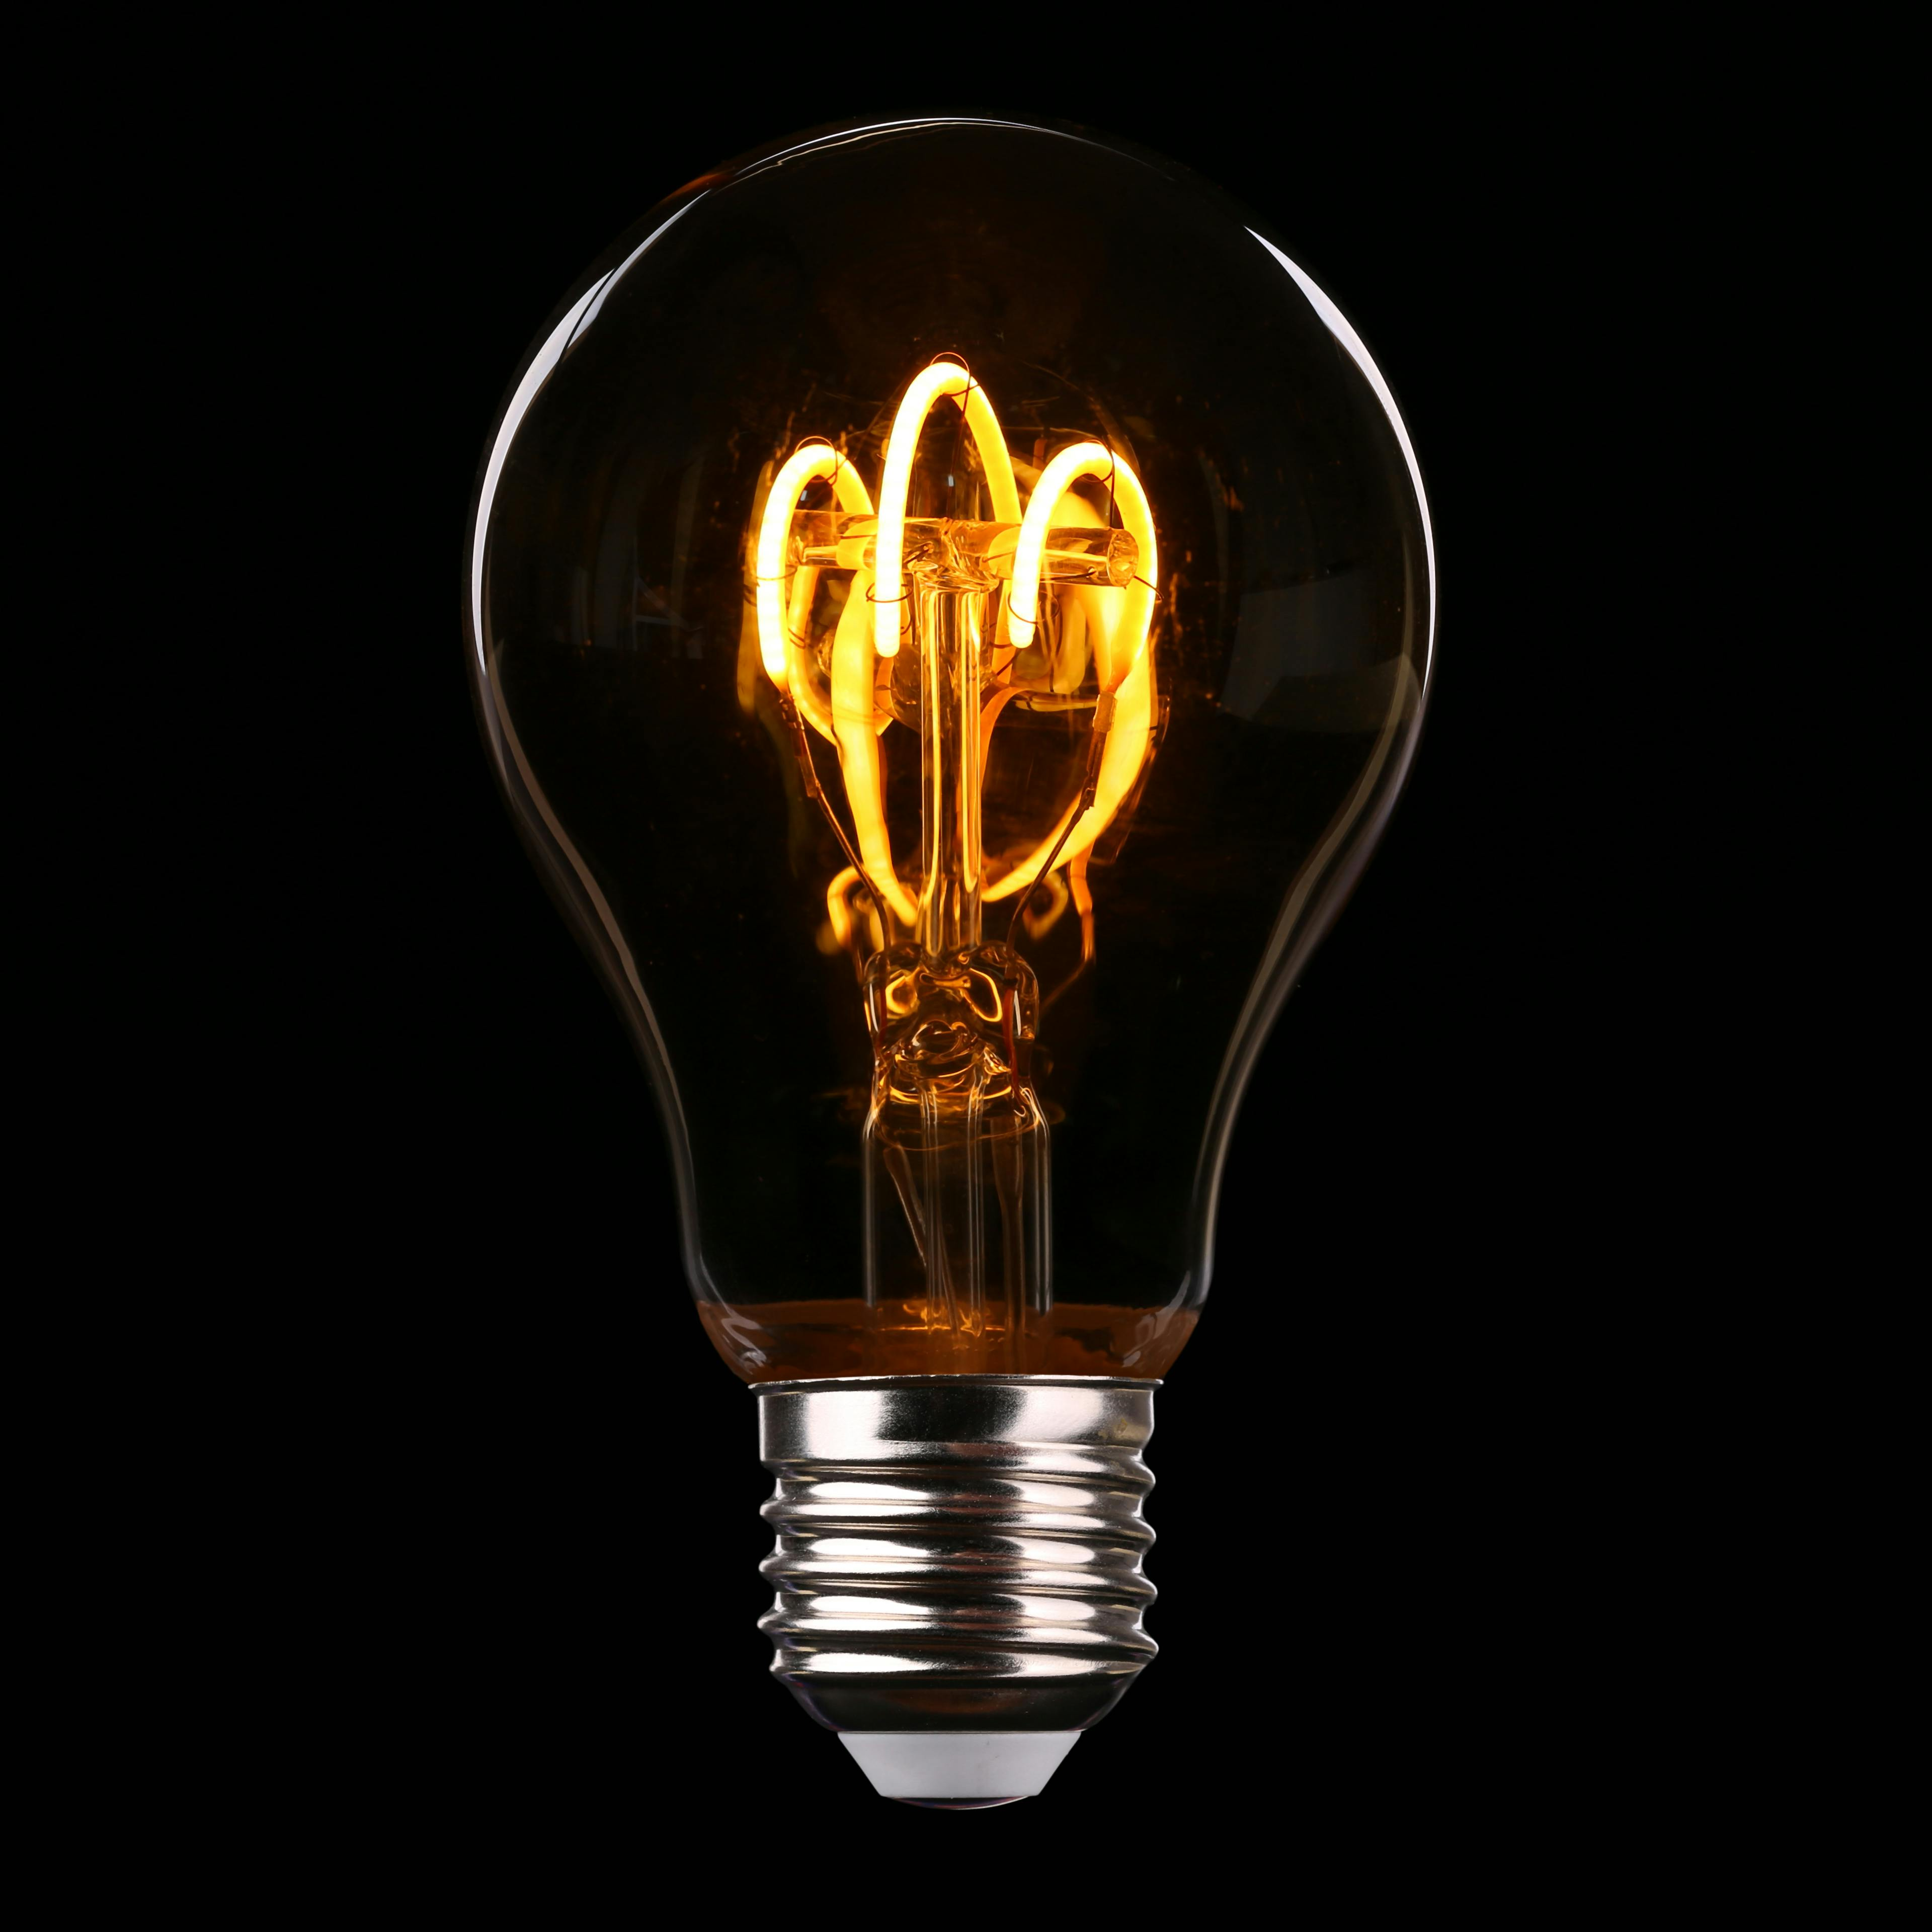
\includegraphics[width=0.7\linewidth, frame]{img/figure.jpg}
	\caption{Lorem ipsum dolor sit amet, consetetur sadipscing elitr, sed diam nonumy eirmod tempor invidunt}
	\label{fig:first_figure}
\end{figure}





\newpage
\sloppy 
\printbibliography

\end{document}